\documentclass[12pt,a4paper,article,english,firamath]{nsi}
\pagestyle{empty}
\setfontfamily{\brettley}{Cursive standard}[Scale=1.5]
\begin{document}
\titre{Find your figure}
\classe{Euro 1\ere}
\maketitle

\subsection*{Description 9}
{\brettley 

Draw one line segment and the two other line segments passing through the endpoints of the first one, perpendicularly to it. The new segments should have the same length as the initial one and be on the same side of it. Join the second endpoints of the two new segments. Draw a line segment joining two of the four points, diagonally. Place the midpoint of this line segment. Draw a line parallel to the initial line segment, passing through this point. Finally, draw a circle passing through the midpoints of the first four segments.}\\[1em]

\begin{tikzpicture}
    \draw[lightgray](0,0)--(\linewidth,0);
\end{tikzpicture}


\subsection*{Figure 9}
\begin{center}
    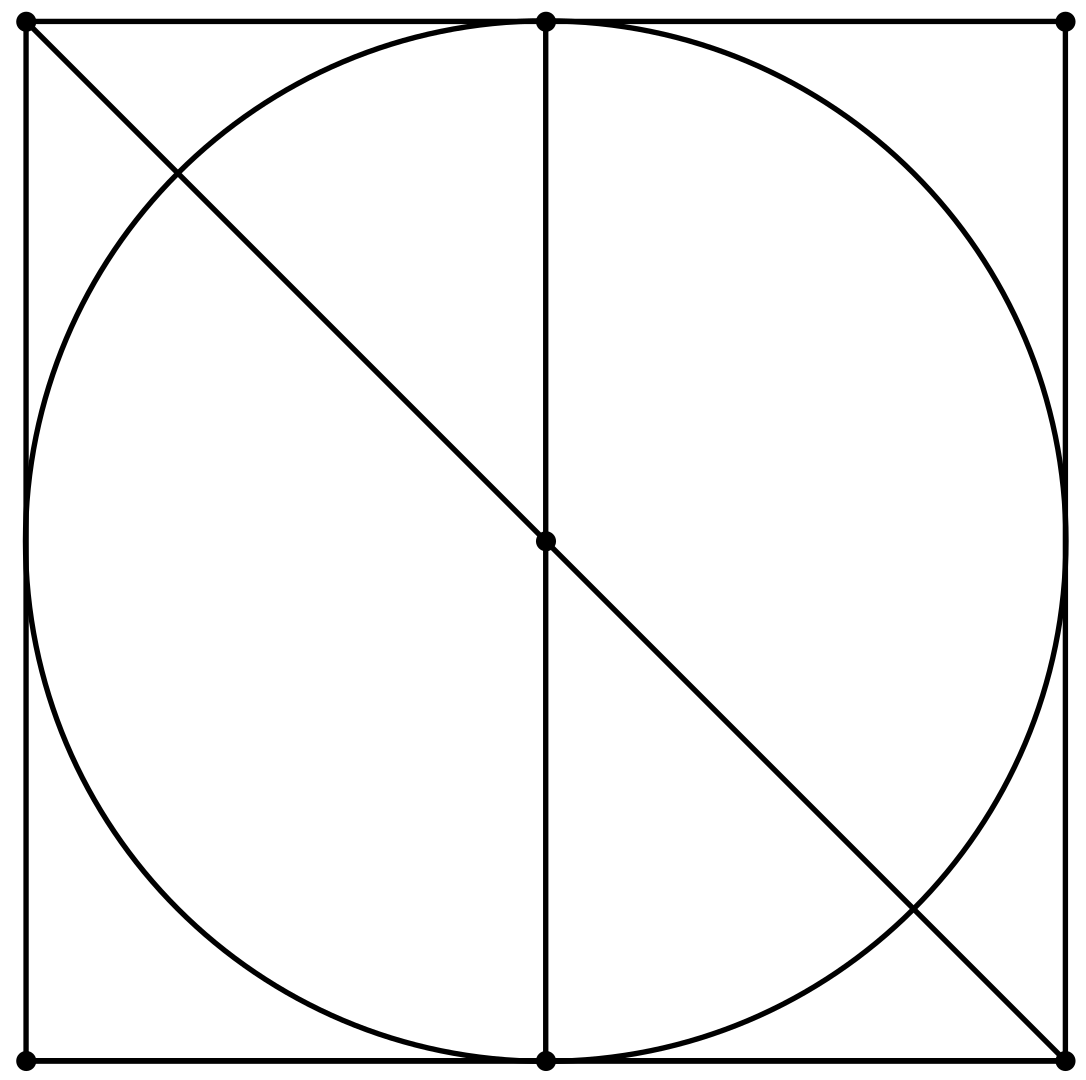
\includegraphics[height=10cm]{img/fig09.png}
\end{center}
\end{document}